\documentclass[conference]{IEEEtran}

\usepackage{amsmath}
\usepackage{booktabs}
\usepackage{graphicx}
\usepackage{microtype}
\usepackage{url}

\title{AnnotateBench: A Cost-Aware Benchmark for Label-Efficient Text Classification}

\author{
\IEEEauthorblockN{Aitong Zhang, Natan Vidra, Spurthi Setty}
\IEEEauthorblockA{\textit{Anote AI}\\
USA\\
\{az535@cornell.edu, nvidra@anote.ai, ssetty2@stevens.edu\}}
}

\begin{document}
\maketitle

\begin{abstract}
Large data pipelines often have abundant unlabeled records but scarce, expensive, or unreliable labels. We present AnnotateBench, a reproducible benchmark that evaluates which text examples to label, how many labels to acquire, and how annotation source affects downstream utility and direct cost. Its primary study contains 1,000 conditions spanning ten datasets, four selection strategies, five budgets, and five seeds; three human-cost scenarios produce 3,000 auditable cost records. No strategy is uniformly best, and exploratory paired tests do not establish a universal winner after multiplicity correction. Secondary studies show that rankings depend on downstream representation and on whether acquisition is one-shot or cumulative. An AG News stress test measures selection---not end-to-end processing---for pools up to 10,000 candidates. A three-seed LLM extension compares generated and gold labels on exactly the same examples: generated labels reduce mean downstream macro F1 on eight of ten datasets, including tasks with over 90\% label agreement; the two positive mean gaps are small relative to seed variation. AnnotateBench therefore connects annotation volume, veracity, and value while exposing the assumptions behind each recommendation.
\end{abstract}

\begin{IEEEkeywords}
data-centric AI, big data benchmarks, data annotation, active learning, text classification
\end{IEEEkeywords}

\section{Introduction}

Data acquisition decisions shape the quality and cost of machine-learning systems. In big-data pipelines, the central imbalance is often not a shortage of raw records but an abundance of unlabeled records and a shortage of trustworthy labels. For supervised text classification, teams must choose which examples to label, how many labels to buy, and whether labels should come from people or language models. These choices are usually evaluated in isolated studies at one budget, making it difficult to distinguish early gains from diminishing returns or to compare quality with direct annotation cost.

AnnotateBench treats annotation strategy selection as a benchmark problem. Given an unlabeled training pool and budget, a strategy chooses examples; labels are then revealed or generated, a fixed downstream classifier is trained, and performance is measured on a held-out gold test set. Repeating this protocol across budgets produces learning curves and cost--performance frontiers rather than a single score. In the five-V vocabulary of big data, the benchmark probes \emph{volume} through pool scaling, \emph{variety} through ten datasets, \emph{veracity} through human-versus-LLM labels, \emph{value} through downstream utility per dollar, and \emph{velocity} through measured selection time. It does not equate a 10,000-example stress test with web-scale processing; instead, it makes the scaling boundary measurable.

The benchmark is designed as a data-centric AI evaluation framework, not as a new active-learning algorithm. Its contributions are:
\begin{itemize}
    \item a controlled evaluation over ten text-classification datasets, four gold-label selection strategies, five budgets, and five seeds;
    \item direct-cost models and Pareto analyses that convert learning curves into budget-allocation evidence;
    \item paired statistical comparisons, fixed-budget and nested acquisition protocols, and a pool-scaling runtime study;
    \item a downstream-model sensitivity comparison that keeps acquisition in TF--IDF space while changing the final representation; and
    \item an API-backed LLM annotation extension that distinguishes label agreement from downstream training utility.
\end{itemize}

The implementation, camera-ready analysis, corrected results, and validation scripts are available in the public repository.\footnote{\url{https://github.com/anote-ai/Research-AnnotateBench/tree/feature/benchmark-robustness-scalability}}

\section{Related Work}

\subsection{Data-Centric Evaluation}
DataPerf formalizes data selection, acquisition, and debugging as benchmark tasks \cite{mazumder2022dataperf}; related acquisition benchmarks emphasize transparent pricing and standardized interactions \cite{chen2023dataacquisition}. DataComp evaluates curation under a fixed training pipeline at multimodal scale \cite{gadre2023datacomp}, while OpenDataVal compares data-valuation algorithms \cite{jiang2023opendataval}. AnnotateBench adds a narrower operational capability not jointly covered by those suites: evaluating text-example acquisition policy, annotation source, monetary cost, and the utility of the resulting trained classifier across multiple label budgets.

Table~\ref{tab:positioning} makes that distinction explicit. DataPerf is a broad collection of data-centric challenges, DataComp studies large-scale multimodal filtering, and OpenDataVal evaluates the value assigned to existing points. AnnotateBench instead links text example acquisition, annotation source, monetary cost, and the utility of the resulting trained model. The comparison is about benchmark scope, not a claim that one suite supersedes another.

\begin{table*}[t]
\caption{Scope comparison with adjacent data-centric benchmarks. A dash means the feature is outside the benchmark's principal reported scope.}
\label{tab:positioning}
\centering
\footnotesize
\setlength{\tabcolsep}{2pt}
\begin{tabular}{lccccccl}
\toprule
Benchmark & Primary task & Text labels & Multiple budgets & Human/LLM source & Monetary cost & Downstream utility & Pareto/target analysis \\
\midrule
DataPerf \cite{mazumder2022dataperf} & data-centric challenges & some & task-dependent & -- & task-dependent & yes & -- \\
DataComp \cite{gadre2023datacomp} & multimodal filtering & -- & compute scales & -- & compute budget & yes & scaling laws \\
OpenDataVal \cite{jiang2023opendataval} & data valuation & yes & training-set sizes & -- & -- & yes & -- \\
AnnotateBench & label acquisition & yes & 5 & human + LLM & yes & yes & yes \\
\bottomrule
\end{tabular}
\end{table*}

\subsection{Active and LLM-Assisted Annotation}
Few-shot text classification and continuous human feedback show that small labeled sets can be useful \cite{tunstall2022setfit,vidra2024humanfeedback}. Active annotation additionally studies which examples should receive those labels; recent work combines LLM outputs with human annotation and cost-aware selection \cite{rouzegar2024llmdriven}. LLM-as-annotator studies report promising label agreement and cost reductions \cite{wang2021gpt3labeling,gilardi2023chatgpt,pangakis2024distillation}, but agreement alone does not establish the utility of generated labels for training. AnnotateBench compares budgeted selection, annotation source, downstream performance, and direct cost under one protocol.

\section{Benchmark Design}

\subsection{Problem Setup}
Let $D_{\mathrm{train}}=\{(x_i,y_i)\}_{i=1}^{n}$ be a public labeled training set and $D_{\mathrm{test}}$ a held-out gold test set. A strategy $s$ receives the training inputs and a budget $b$, then selects $S_{s,b}$ with $|S_{s,b}|\le b$. For the gold-label benchmark, dataset labels simulate human annotation: random and diversity selection use no labels, whereas uncertainty and hybrid reveal initial-set labels before selecting the remaining batch. All revealed labels count toward the budget. A classifier trained on $S_{s,b}$ is evaluated on $D_{\mathrm{test}}$ using macro F1 and accuracy.

The primary protocol treats each budget as an independent experimental condition rather than a prefix of one continuous acquisition trajectory. This is the intended setting for a team choosing a one-time annotation batch: it compares the attainable quality of policies at the specified budget without allowing an earlier allocation to constrain a later one. Because deployed active learning normally reuses labels, we also run nested cumulative trajectories on Financial PhraseBank, TREC, and Yelp Polarity. The two protocols answer different questions and are reported separately.

\subsection{Selection and Annotation Strategies}
We evaluate uniform random sampling; entropy-based uncertainty sampling; farthest-first diversity sampling in TF--IDF space; and a hybrid policy. For uncertainty, a random initial set of size $\min(\max(2,\lfloor b/10\rfloor),b,n)$ is labeled and counts toward budget and cost. If it contains at least two observed classes, one TF--IDF logistic-regression model ranks all remaining points by entropy and the rest of the budget is selected in a single batch, without iterative retraining. Otherwise, the selector falls back to random completion. Thus, the seed is not class-covering---which would be impossible for Banking77's 77 classes at a 50-label budget. Hybrid first selects half the budget by TF--IDF diversity, then performs the same single uncertainty batch.

\begingroup\raggedright The LLM extension uses nested random budgets. API responses identify model \texttt{gpt-4o-mini-2024-07-18}. The prompt identifier is \texttt{text\_classification\_v1\_zero\_shot\_json}; temperature is 0 and JSON-object output is requested. After JSON decoding, unsupported labels or invalid annotation fields trigger assignment of the first permitted label with confidence zero. JSON decoding failures propagate as errors rather than using this fallback. Two invalid-label outputs occur in the available seed-1/2 caches, both for Banking77; seed-0 row-level responses are unavailable. The final classifier is trained on generated rather than gold labels. At budget 250, nested random indices coincide with the existing same-seed random gold runs, whose classifier results are reused as the matched comparator; the best observed gold selector is retained only as a separate retrospective reference.\par\endgroup

Selection is repeated independently for every $(s,b,\mathrm{seed})$ condition in the primary grid. In particular, the 100-label set is not guaranteed to contain the 50-label set. For the cumulative variant, random and diversity policies create one ordered acquisition list, while uncertainty and hybrid policies expand the currently labeled set at each budget. The artifact checks that every smaller set is a strict subset of the next set. Costs at a cumulative endpoint describe all labels acquired up to that endpoint; they are not summed again across intermediate checkpoints.

\subsection{Learning Curves and Costs}
For every strategy--budget pair, AnnotateBench records performance and direct annotation cost. Human cost is a sensitivity parameter with low, base, and high scenarios derived from public requester pricing pages checked July 12, 2026.\footnote{\url{https://www.mturk.com/pricing}; \url{https://www.prolific.com/pricing}} The corresponding per-label costs are \$0.040, \$0.0952, and \$0.4284; reported table costs use these unrounded inputs. They combine an hourly reward assumption, estimated task time, platform fee, and label redundancy; they are intended for sensitivity analysis rather than as a universal price. Under human-label cost $h$ and strategy overhead $o_s$,
\begin{equation}
C(s,b)=(h+o_s)|S_{s,b}|.
\end{equation}
Base selection overhead is \$0 for random, \$0.002 for uncertainty, \$0.003 for diversity, and \$0.004 for hybrid. These are explicit scenario assumptions, not measured production invoices.

For token counts $t_{\mathrm{in}},t_{\mathrm{out}}$ and prices checked July 22, 2026 (\$0.15 and \$0.60 per million input and output tokens), LLM API cost is
\begin{equation}
C_{\mathrm{LLM}} =
\frac{t_{\mathrm{in}}p_{\mathrm{in}}+t_{\mathrm{out}}p_{\mathrm{out}}}{10^6}.
\end{equation}
Historical seed-1/2 cost summaries use recorded token counts; these summaries are retained after the FPB label repair rather than remeasuring the corrected batch cost. Seed 0 predates complete logging, so its total is estimated with a deterministic 30-example length-stratified sample per dataset. Retrospective validation on complete seed-1/2 logs gives 2.44\% mean absolute percentage error.

A point is Pareto-efficient if no alternative has no greater cost and no lower macro F1, with at least one strict improvement.

\begin{table}[t]
\caption{Primary reported quantities and their roles.}
\label{tab:metrics}
\centering
\footnotesize
\begin{tabular}{lp{0.62\columnwidth}}
\toprule
Quantity & Interpretation \\
\midrule
Macro F1 & Class-balanced downstream test utility \\
Label accuracy & Agreement of LLM labels with dataset labels \\
Total cost & Modeled annotation plus selection cost \\
Target cost & Lowest evaluated-grid cost attaining a score \\
Pareto efficiency & No point has no greater cost and no lower F1, with at least one strict improvement \\
Selection time & Selector wall time only; not end-to-end latency \\
\bottomrule
\end{tabular}
\end{table}

\subsection{Computational Scope}
Random selection is linear in pool size. Uncertainty selection fits and scores one sparse classifier per budget. The implemented farthest-first diversity policy repeatedly computes distances from the pool to the growing selected set; its unoptimized worst-case work grows quadratically in the budget and linearly in pool size. Consequently, the present study caps large training pools and should be read as an annotation-budget benchmark, not as evidence that every policy scales to unrestricted corpora.

\section{Experimental Setup}

\subsection{Datasets}
The suite covers sentiment, emotion, topic, question-type, and intent classification: Financial PhraseBank \cite{malo2014good}, TREC coarse \cite{li2002learning}, Banking77 \cite{casanueva2020efficient}, AG News and Yelp Polarity \cite{zhang2015character}, SST-2 \cite{socher2013recursive}, 20 Newsgroups \cite{lang1995newsweeder}, Rotten Tomatoes \cite{pang2005seeing}, TweetEval Sentiment \cite{barbieri2020tweeteval}, and Emotion \cite{saravia2018carer}. Financial PhraseBank uses a deterministic stratified 80/20 split; TREC, Banking77, and the remaining Hugging Face datasets use their public splits. Training pools are capped at 1,200 examples and test sets at 1,000 to keep repeated selection tractable.

\begin{table}[t]
\caption{Benchmark suite after deterministic caps. ``FPB'' denotes Financial PhraseBank and ``20NG'' denotes 20 Newsgroups.}
\label{tab:datasets}
\centering
\footnotesize
\begin{tabular}{lrrl}
\toprule
Dataset & Classes & Train/test & Task \\
\midrule
AG News & 4 & 1200/1000 & topic \\
Banking77 & 77 & 1200/1000 & intent \\
Emotion & 6 & 1200/1000 & emotion \\
FPB & 3 & 1200/453 & sentiment \\
Rotten Tomatoes & 2 & 1200/1000 & sentiment \\
SST-2 & 2 & 1200/1000 & sentiment \\
TREC & 6 & 1200/500 & question type \\
TweetEval Sentiment & 3 & 1200/1000 & sentiment \\
20NG & 20 & 1177/973 & topic \\
Yelp Polarity & 2 & 1200/1000 & sentiment \\
\bottomrule
\end{tabular}
\end{table}

\subsection{Models, Budgets, and Repetition}
The primary downstream learner is TF--IDF over unigrams and bigrams followed by logistic regression. This controlled learner isolates strategy effects rather than pursuing state-of-the-art accuracy. The vectorizer and classifier use the versioned repository defaults; the classifier random state is tied to the experimental seed. A downstream-model sensitivity study replaces only the final classifier's sparse features with frozen \texttt{all-MiniLM-L6-v2} sentence embeddings while retaining logistic regression. Selection still uses the original TF--IDF diversity representation and TF--IDF uncertainty learner; the experiment does not test embedding-based acquisition.

Gold-label experiments use budgets 50, 100, 250, 500, and 1,000 and seeds 0--4. Ten datasets, four strategies, five budgets, and five seeds create 1,000 experimental conditions. Attaching three cost scenarios creates 3,000 records without tripling model fits. The LLM extension uses budgets 50, 100, and 250 and seeds 0--2.

Macro F1 is primary because the suite includes high-cardinality and imbalanced tasks; accuracy is retained in the artifact. Tables report arithmetic means over seeds. The 95\% intervals use the small-sample Student-$t$ critical value $t_{.975,4}=2.776$ times $s/\sqrt{5}$ and describe run-to-run variation under the five selected seeds. They are not formal pairwise hypothesis tests, and failure to reject a difference is not evidence of equivalence. We therefore treat overlapping intervals as a reason for caution and do not convert small rank differences into significance claims.

For a stronger exploratory comparison, we identify each dataset's two highest mean-performing strategy--budget configurations and compute their within-seed macro-F1 differences. We report the paired mean, a 20,000-resample paired bootstrap interval, paired standardized effect $d_z$, and an exact two-sided sign-flip test over the five seed differences. Holm adjustment controls the family of ten dataset-level tests. Because configurations are chosen on the same grid and $n=5$ gives a minimum attainable two-sided exact $p$ of .0625, these analyses quantify uncertainty rather than establish confirmatory superiority.

The cumulative study uses the same five budgets, five seeds, learner, and 1,200-example caps on three representative datasets. The volume study separately loads a deterministic AG News sample, fixes the label budget at 100, and expands the candidate pool from 1,200 to 5,000 and 10,000 examples. It records wall-clock selection time and downstream performance over three seeds on an Apple Silicon machine. Runtime is implementation- and hardware-specific; its purpose is to reveal growth and the current operating range, not to claim distributed-system throughput.

\subsection{Reproducibility}
Dataset loaders, selection policies, model parameters, result-generation scripts, aggregate CSV files, and validation checks are versioned with the artifact. The result-generating analysis revision is \texttt{a4d29d0}, available on branch \texttt{feature/benchmark-robustness-scalability}. Random seeds are explicit. The main entry point is \texttt{scripts/run\_benchmark.py}; \texttt{scripts/validate\_benchmark\_results.py} checks the 3,000-row gold-label grid. Separate scripts regenerate the five-seed downstream-model comparison, paired statistics, nested trajectories, scalability study, matched-gold analysis, cost sensitivities, and paper figures. Generated CSVs retain dataset, strategy, budget, seed, model or trajectory type, and cost provenance. Public gold labels simulate annotation; no new human-subject data were collected.

\section{Results}

\subsection{Gold-Label Benchmark}

\begin{table*}[t]
\caption{Best gold-label strategy--budget point per dataset under the base cost scenario. Scores are mean macro F1 with 95\% confidence intervals over five seeds.}
\label{tab:gold}
\centering
\scriptsize
\setlength{\tabcolsep}{3pt}
\begin{tabular}{lcrrr@{\hspace{0.8em}}lcrrr}
\toprule
Dataset & Strategy & Labels & Macro F1 & Cost &
Dataset & Strategy & Labels & Macro F1 & Cost \\
\midrule
AG News & Hybrid & 1000 & .793 [.782,.804] & \$99.20 &
FPB & Uncertainty & 500 & .755 [.736,.773] & \$48.60 \\
Banking77 & Random & 1000 & .545 [.536,.553] & \$95.20 &
Rotten Tomatoes & Diversity & 1000 & .689 [.676,.702] & \$98.20 \\
Emotion & Hybrid & 1000 & .234 [.227,.240] & \$99.20 &
SST-2 & Uncertainty & 1000 & .712 [.697,.727] & \$97.20 \\
TREC & Hybrid & 1000 & .788 [.784,.791] & \$99.20 &
TweetEval & Hybrid & 1000 & .360 [.352,.368] & \$99.20 \\
20NG & Random & 1000 & .348 [.307,.389] & \$95.20 &
Yelp Polarity & Hybrid & 1000 & .868 [.845,.890] & \$99.20 \\
\bottomrule
\end{tabular}
\end{table*}

No strategy dominates across datasets (Table~\ref{tab:gold}). Hybrid leads on five datasets, random and uncertainty on two each, and diversity on one. The result is not a universal ranking: top-two Student-$t$ intervals overlap on seven datasets, including Emotion, so small differences should be treated as non-definitive rather than as significance tests. The paired analysis sharpens this caution. Mean top-two gaps range from .0008 to .0410 macro F1; five paired bootstrap intervals exclude zero, but none of the ten exact sign-flip comparisons survives Holm correction (minimum adjusted $p=.625$). With five seeds and post-selection of the top two configurations, the evidence supports heterogeneous practical effects, not a statistically resolved universal winner; non-significance does not establish equivalence.

As retrospective summaries of the evaluated grid, learning curves (Fig.~\ref{fig:learning}) reveal different target-attainment costs; they are not deployable rules available without validation or test feedback. Under the base scenario, Financial PhraseBank reaches macro F1 .50 with 100 hybrid-selected labels (\$9.92) and .75 with 500 uncertainty-selected labels (\$48.60). Yelp Polarity reaches .75 with 500 random labels (\$47.60), but diversity is the least expensive evaluated option reaching .80 (\$49.10).

The controlled learner also exposes task difficulty that selection alone cannot solve. Under the 1,000-label cap, Emotion, TweetEval Sentiment, and 20 Newsgroups remain below .50 macro F1, whereas Yelp Polarity exceeds .80. Banking77 illustrates the effect of label cardinality: even 1,000 labels cover 77 intents sparsely, and random sampling remains best in this grid. These results motivate reporting the entire budget curve rather than only the endpoint.

\begin{figure}[t]
\centering
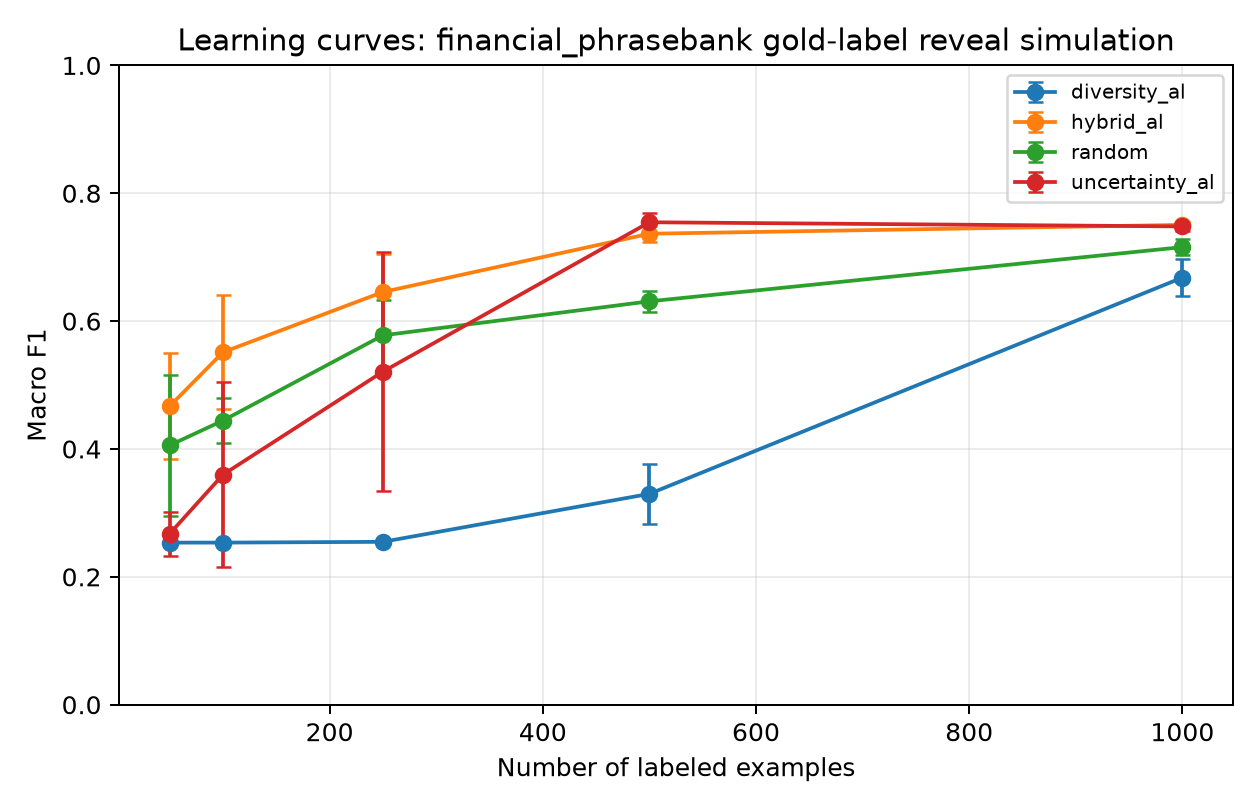
\includegraphics[width=\columnwidth]{figures/learning_curve_financial_phrasebank.png}
\caption{Financial PhraseBank learning curves under the base human-cost scenario. Error bars show one sample standard deviation across five seeds.}
\label{fig:learning}
\end{figure}

\subsection{Fixed Budgets Versus Cumulative Acquisition}
Across the three trajectory datasets and five budgets, the best strategy agrees between the independent and nested protocols in 11 of 15 comparisons. The disagreement is operationally meaningful at the 1,000-label endpoint for TREC and Yelp Polarity (Table~\ref{tab:cumulative}). For TREC, hybrid leads the independent grid at .788, whereas random leads the cumulative trajectory at .767. For Yelp, hybrid reaches .868 when selected afresh at 1,000 labels, while diversity leads the cumulative path at .827. Financial PhraseBank is stable at the endpoint, although its winners differ at the two smallest budgets. Thus, a fixed-budget benchmark estimates a fresh allocation decision; it should not be described as the learning history of a deployed system.

\begin{table}[t]
\caption{Best strategy and mean macro F1 at 1,000 labels under independent fixed-budget (F) and nested cumulative (C) protocols.}
\label{tab:cumulative}
\centering
\footnotesize
\begin{tabular}{lcc}
\toprule
Dataset & Fixed (F) & Cumulative (C) \\
\midrule
Financial PhraseBank & H/.751 & H/.754 \\
TREC & H/.788 & R/.767 \\
Yelp Polarity & H/.868 & D/.827 \\
\bottomrule
\end{tabular}
\end{table}

\subsection{Candidate-Pool Scalability}
Figure~\ref{fig:scalability} measures only the selector implementations at a fixed 100-label budget. From 1,200 to 10,000 AG News candidates, mean selection time grows from .070 to .466 seconds for diversity, .061 to .380 for hybrid, and .019 to .144 for uncertainty; random sampling remains below one millisecond on the reported Apple Silicon machine. The sub-.5-second observation excludes annotation latency, final classifier training, and end-to-end pipeline cost. It is bounded evidence rather than a web-scale claim: the label budget is small, the features are sparse, and the current diversity implementation will become expensive as both pool and budget grow. Macro F1 is noisy across the three sampled seeds and does not increase monotonically with candidate-pool size, underscoring that access to more unlabeled data does not guarantee a better 100-point labeled subset.

\begin{figure}[t]
\centering
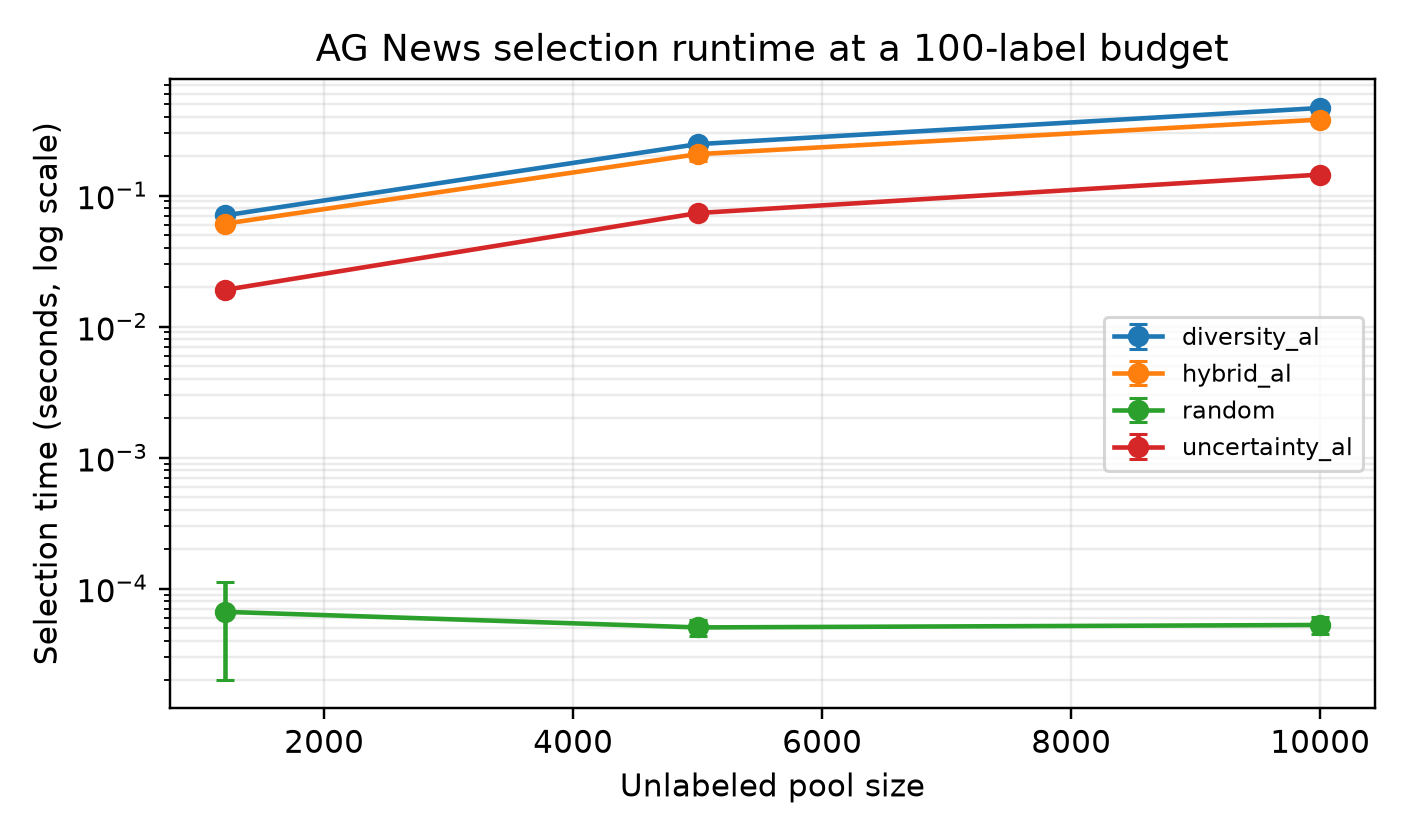
\includegraphics[width=\columnwidth]{figures/pool_scalability_runtime.png}
\caption{AG News selection runtime as the candidate pool grows at a fixed 100-label budget (mean and standard deviation over three seeds; log time axis).}
\label{fig:scalability}
\end{figure}

\subsection{Downstream-Model Sensitivity}
Table~\ref{tab:robustness} shows that the sentence-embedding learner improves the best macro F1 on eight of ten datasets in the five-seed robustness grid, including large gains on 20 Newsgroups, Emotion, TweetEval Sentiment, and Banking77. It is worse on TREC and Yelp Polarity. Best-strategy identity agrees on only five of ten datasets, and the four-strategy rank correlation ranges from $-0.4$ to $1.0$. Thus, the absolute benefit and ranking of an annotation policy depend on the downstream representation; the sparse-model grid is a controlled baseline, not an upper bound.

\begin{table}[t]
\caption{Five-seed downstream-model sensitivity. Acquisition remains in TF--IDF space; only the final representation changes. Entries are the highest mean F1 over the evaluated strategy--budget grid for each downstream model. R, U, D, and H denote random, uncertainty, diversity, and hybrid.}
\label{tab:robustness}
\centering
\footnotesize
\begin{tabular}{lcc}
\toprule
Dataset & TF--IDF & Sentence emb. \\
\midrule
AG News & .793/H & .854/R \\
Banking77 & .545/R & .741/R \\
Emotion & .234/H & .470/H \\
Financial PhraseBank & .755/U & .847/D \\
Rotten Tomatoes & .689/D & .742/D \\
SST-2 & .712/U & .801/H \\
TREC & .788/H & .721/H \\
TweetEval Sentiment & .360/H & .577/R \\
20 Newsgroups & .348/R & .632/R \\
Yelp Polarity & .868/H & .852/R \\
\bottomrule
\end{tabular}
\end{table}

\subsection{LLM Annotation Utility}
At 250 labels, LLM label accuracy varies from .584 on Emotion to .972 on Yelp Polarity. Table~\ref{tab:llm} isolates annotation source by pairing every LLM run with gold labels on exactly the same examples. The matched gaps are noisy over three seeds: Yelp Polarity averages +.035 with SD .060, so it does not establish an LLM advantage. Financial PhraseBank is similarly inconclusive at +.024 with SD .049 despite .929 label accuracy. AG News and TREC retain large matched deficits of $-.235$ and $-.190$. LLM labels reduce mean macro F1 on eight of ten datasets, including Rotten Tomatoes (.908 label accuracy, gap $-.141$) and SST-2 (.921, $-.104$). The available seed-1/2 main-extension caches contain two off-schema outputs, both for Banking77; they cannot directly explain losses on the other datasets. Low downstream scores also warrant caution: some Emotion runs approach a single-class predictor, 20 Newsgroups has mean macro F1 .013, and two budget-250 Rotten Tomatoes seeds have approximately .50 test accuracy. We report these outcomes without attributing them to a specific mechanism.

\begin{table}[t]
\caption{Budget-250 LLM comparison over seeds 0--2. ``Matched'' uses gold labels on the identical random examples. Gap is LLM minus matched macro F1 (mean $\pm$ sample SD). ``Best ref.'' averages the highest test-F1 gold selector among four strategies separately for each seed 0--2 at budget 250; it is not the matched comparator.}
\label{tab:llm}
\centering
\scriptsize
\setlength{\tabcolsep}{2.5pt}
\begin{tabular}{lrrrrr}
\toprule
Dataset & LLM & Matched & Gap $\pm$ SD & Best ref. & Label acc. \\
\midrule
AG News & .404 & .639 & $-.235\pm.047$ & .639 & .819 \\
Banking77 & .084 & .138 & $-.054\pm.013$ & .138 & .661 \\
Emotion & .081 & .147 & $-.066\pm.031$ & .158 & .584 \\
FPB & .589 & .565 & $+.024\pm.049$ & .634 & .929 \\
Rotten Tomatoes & .426 & .567 & $-.141\pm.102$ & .588 & .908 \\
SST-2 & .511 & .616 & $-.104\pm.136$ & .634 & .921 \\
TREC & .338 & .528 & $-.190\pm.032$ & .528 & .691 \\
TweetEval & .236 & .304 & $-.069\pm.041$ & .312 & .668 \\
20NG & .013 & .104 & $-.091\pm.049$ & .107 & .643 \\
Yelp Polarity & .675 & .640 & $+.035\pm.060$ & .672 & .972 \\
\bottomrule
\end{tabular}
\end{table}

Historical mean per-run API cost estimates at budget 250 range from roughly \$0.014 on short sentiment datasets to \$0.048 on Banking77. API cost excludes human review, failed requests, latency, and quality control. Scaling selection overheads by 2, 5, and 10 leaves all ten gold-label Pareto sets unchanged. Figure~\ref{fig:pareto} adds a separate sensitivity scenario that reviews 10\% of LLM labels at the full-precision base rate of \$0.0952 per item: costs increase by \$0.476, \$0.952, and \$2.380 at budgets 50, 100, and 250 without assuming any performance improvement. This is an illustrative cost shift, not an observed production workflow.

\subsection{Row-Level Reliability Diagnostics}
Three separate held-out annotation pilots describe label-error patterns; they do not identify causes of the main training-utility gaps. Each labels 100 test examples at temperatures 0 and 0.7 with three replicates, yielding 600 annotations per dataset. Financial PhraseBank reaches .990 label accuracy and .987 label macro F1; all six errors turn positive examples into neutral ones. TREC reaches .792 accuracy but only .562 macro F1 when schema-external outputs are counted as predicted labels. TweetEval Sentiment reaches .782 accuracy and .766 macro F1, with many errors softening polarized tweets to neutral. Pairwise temperature and replicate comparisons are not significant after Bonferroni correction in these pilots; this does not establish equivalence or stability. The 600 annotations per dataset repeat 100 unique items and are not independent observations. FPB uses a separate dataset-specific prompt, and pilot metrics retain schema-external predictions rather than the main extension's fallback. These pilots do not validate the main protocol or constitute a cross-model reliability benchmark.

\begin{figure}[t]
\centering
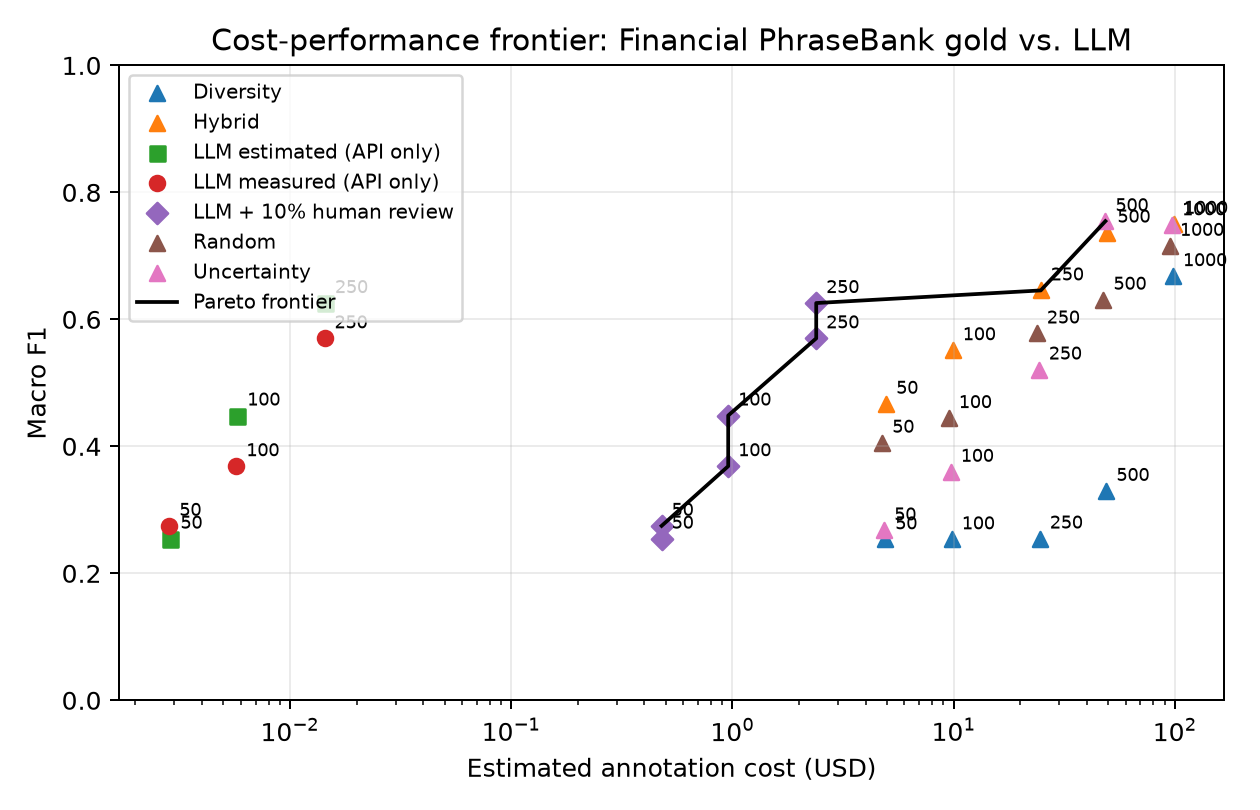
\includegraphics[width=\columnwidth]{figures/pareto_financial_phrasebank.png}
\caption{Financial PhraseBank cost sensitivity. The frontier replaces API-only LLM cost with a scenario reviewing 10\% of generated labels at \$0.0952 each; API-only points remain as reference markers. Performance is held fixed.}
\label{fig:pareto}
\end{figure}

\section{Limitations and Threats to Validity}
Gold-label reveal experiments isolate selection but omit instruction ambiguity, annotator disagreement, interface effects, latency, and adjudication. Public dataset labels are treated as gold even though some tasks contain ambiguity. Human costs are scenario assumptions rather than observed invoices, and LLM costs exclude review and quality control. The three cost scenarios make price sensitivity visible, but they do not substitute for an end-to-end production cost study.

The four selectors cover canonical random, informativeness, coverage, and combined policy families, but they omit newer acquisition baselines and are not an exhaustive active-learning leaderboard. Primary training pools are capped at 1,200 examples because the reference diversity implementation is not optimized for unrestricted scale; the 10,000-candidate runtime study covers only AG News, a 100-label budget, and one machine. The primary learner is deliberately simple to provide a controlled comparison, and the downstream-model study shows sensitivity rather than validating TF--IDF as a production optimum. The LLM extension covers one model snapshot, one prompt family, and three seeds, while its seed-0 token cost is estimated rather than logged. Seed-0 sample matching is reconstructed from the deterministic sampling rule rather than verified against saved row-level responses. Its conclusions should not be generalized to other providers, prompts, decoding settings, or schema-enforcement systems. Finally, all tasks are English text classification, so the findings do not directly generalize to structured prediction, generation, multilingual data, or other modalities.

\section{Conclusion}
AnnotateBench provides a reproducible, cost-aware framework for evaluating annotation choices as budget-allocation decisions in data-intensive pipelines. Across ten datasets, no gold-label selection policy is uniformly best; target attainment, strategy ranking, and diminishing returns depend on the dataset, budget, downstream model, and whether acquisition is one-shot or cumulative. These observations motivate five evaluation practices: select policies per dataset and downstream model; treat agreement as a diagnostic rather than the objective; include review cost before declaring LLM labels Pareto-efficient; match one-shot or nested protocols to the purchase process; and report pool scaling separately from label-budget scaling. The 10,000-candidate stress test makes the current implementation's limited selection-time boundary visible. Matched comparisons show lower mean downstream macro F1 with LLM labels on eight of ten datasets, including tasks with over 90\% label agreement. Positive mean gaps on Financial PhraseBank and Yelp Polarity are small relative to seed variation and do not establish an LLM advantage. Low estimated API cost and high label agreement therefore do not ensure comparable downstream utility. The two main-extension off-schema outputs in the available caches cannot directly explain losses on the other datasets. The benchmark and artifact connect volume, veracity, and value under a shared protocol while exposing the assumptions behind each retrospective recommendation.

\bibliographystyle{IEEEtran}
\bibliography{references}

\end{document}
